\documentclass[12pt,a4paper,twoside]{article}
\usepackage{labor}
\begin{document}

%fill for cover and header creation
\newcommand\laboratorynumber{2}
\title{Abbe-Theorie}
\newcommand\supervisor{Robert Nuster}
\newcommand\groupnumber{42}

\newcommand\participantonelastname{Eisner}
\newcommand\participantonefirstname{Nico}
\newcommand\participantoneid{12214121}
\newcommand\participanttwolastname{Waldl}
\newcommand\participanttwofirstname{Philip}
\newcommand\participanttwoid{12214120}
\author{\participantonelastname \ \& \participanttwolastname}

\newcommand\degreeid{UB 033 678}
\newcommand\semester{23WS}
\date{01.12.2023}

%select correct course title
%\newcommand\coursetitle{Einführung in die \\ physikalischen Messmethoden}
%\newcommand\coursetitle{Laborübungen 1: \\ Mechanik und Wärme}
\newcommand\coursetitle{Laborübungen 2: \\ Elektrizität, Magnetismus, Optik}
%\newcommand\coursetitle{Fortgeschrittenen Praktikum 1: \\ Technische Physik}
%\newcommand\coursetitle{Fortgeschrittenen Praktikum 2: \\ Allgemeine Physik}

%\begin{titlepage}
   \begin{center}
       \begin{figure}[H]
            \begin{minipage}[h]{30mm}
                \centerline{
\includegraphics[height=15mm]{cover_nudes/tugraz.png}}
            \end{minipage}
            \hfill
            \begin{minipage}[h]{30mm}
                \centerline{
\includegraphics[height=15mm]{cover_nudes/nawi_graz.png}}
            \end{minipage}
            \hfill
            \begin{minipage}[h]{30mm}
                \centerline{
\includegraphics[height=15mm]{cover_nudes/uni-graz.png}}
            \end{minipage}
        \end{figure}
        
        \large{\emph{Institut für Experimentalphysik der Technischen Universität Graz \\
        \& Institut für Physik der Universität Graz}} \\
        \vspace{5mm}
        
        {\Huge \textbf{\coursetitle}}
        \vspace{5mm}
        
        {\huge \laboratorynumber: \thetitle}
    \end{center}
    
    \vfill
    
    \begin{table}[H]
        \LARGE
        \centering
        \begin{tabular}{r l}
            Betreuer:       & \supervisor \\
            Gruppennummer:  & \groupnumber \\
            \\
            Name:           & \participantonelastname, \participantonefirstname \\
            Matrikelnummer: & \participantoneid \\
            Name:           & \participanttwolastname, \participanttwofirstname \\
            Matrikelnummer: & \participanttwoid \\
            \\
            Kennzahl:       & \degreeid \\
            Datum:          & \semester \ | \thedate
        \end{tabular}
    \end{table}
    \vspace{4cm}
\end{titlepage}
\clearpage
\setcounter{page}{1}

%\maketitle %short title alternative

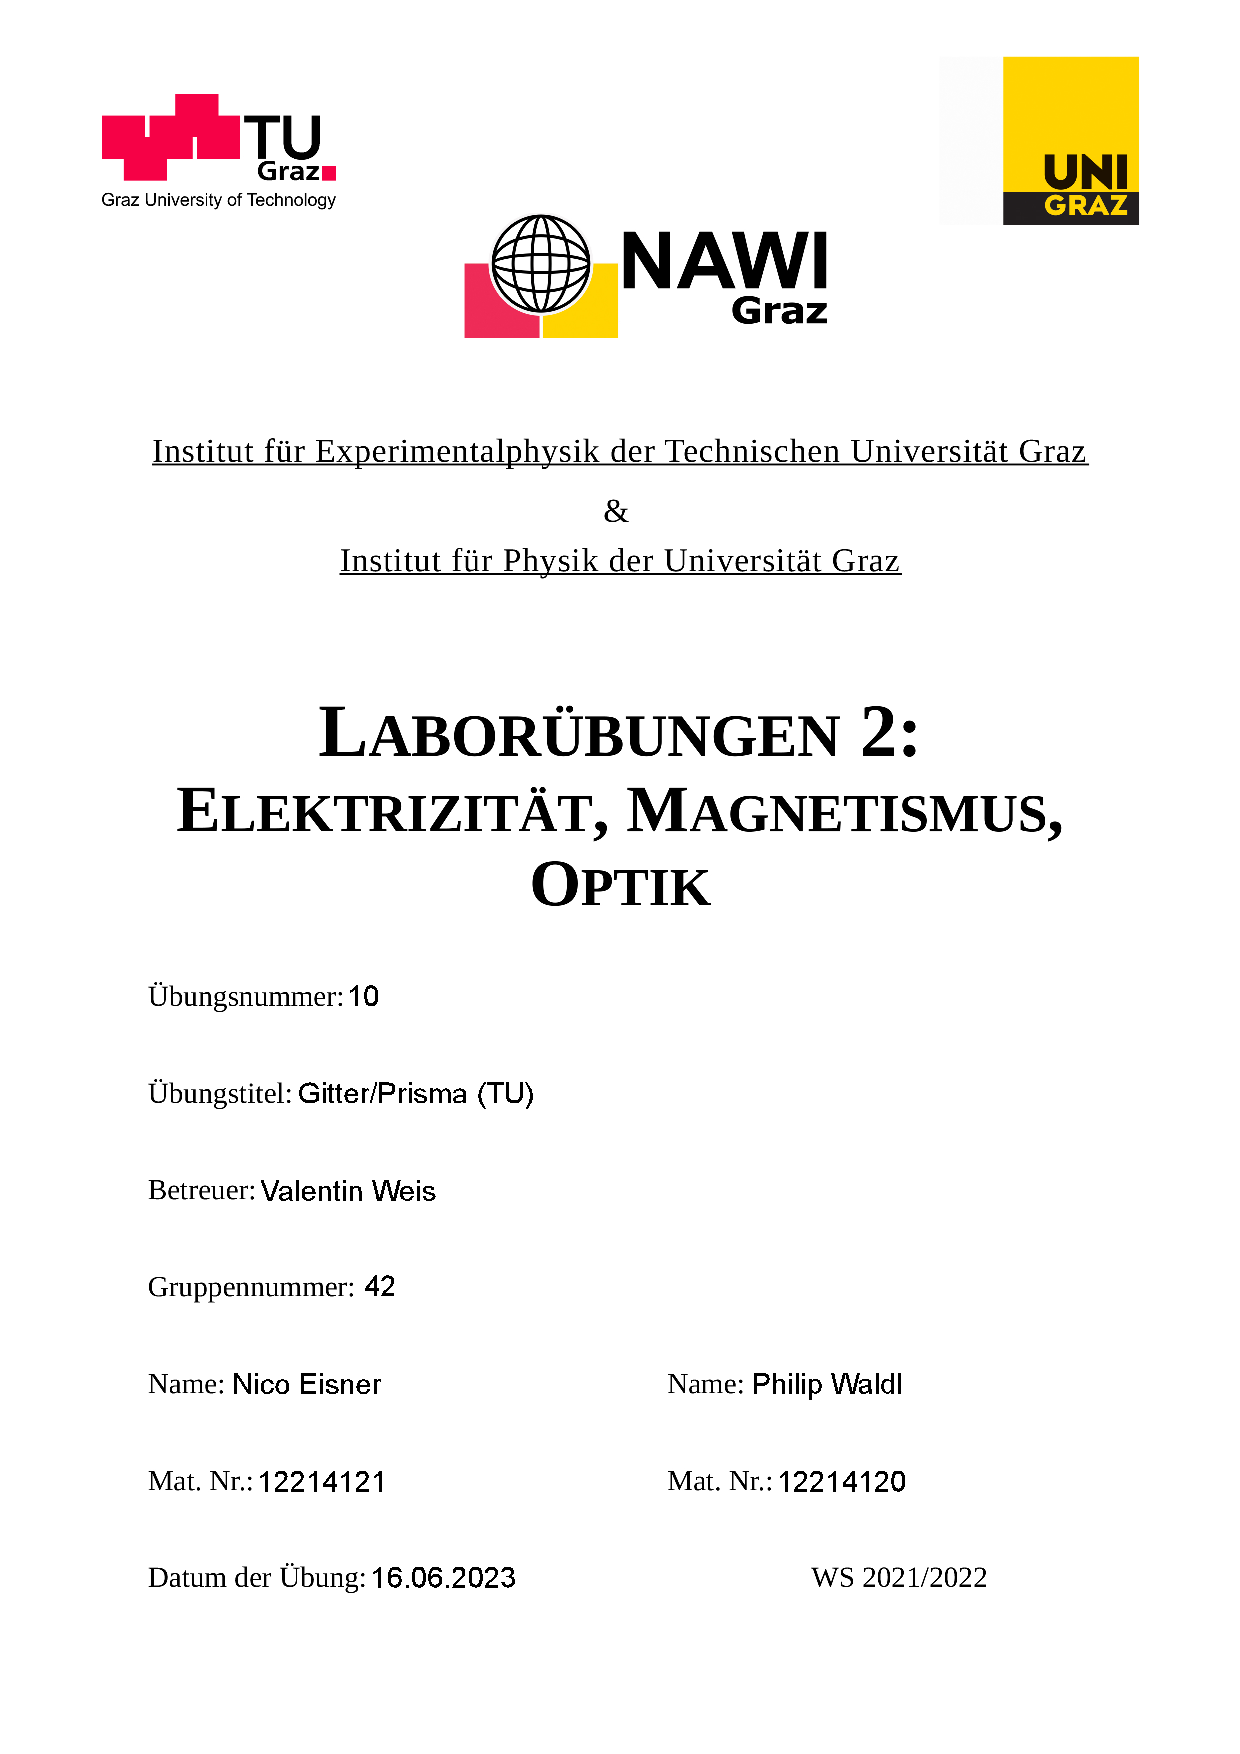
\includepdf[pages={1}]{../Deckblätter/Deckblatt_Gitter.pdf}

\tableofcontents
\newpage

\section{Aufgabenstellung} %jo beschreibn wos gmocht host ------------------------------

Der Versuch Abbe-Theorie behandelt, wie aus dem Namen bereits hervorgeht, die gleichnamige Idee von Ernst Abbe, die in erster Linie die von allen Objekten hervorgehenden Beugungseffekte und deren Zusammenhang mit dem Auflösungsverhalten beinhaltet.
Mittels Experiment der Abbe-Theorie soll dies- und einige weitere Eigenschaften dieses Verhaltens nun gezeigt werden.
Die genauen Arbeitsaufträge sehen dabei wie folgt aus:

\begin{itemize}
    \item Vertrautmachen mit dem experimentellen Aufbau
    \item Bestimmung des Auflösungsvermögens einer Linse in Abhängigkeit ihrer numerischen Apertur für
    \begin{itemize}
        \item blaues Licht
        \item rotes Licht
    \end{itemize}
    \item Untersuchung des Zusammenhangs zwischen der Bildauflösung von einem Spaltgitter und der Zahl der transmittierten Beugungsordnungen
    \item  Freies Experimentieren
    \begin{itemize}
        \item Beugungsbild horizontaler Balken
        \item Änderung des Beugungsbild mit dem Abstand der Balken
        \item Grund für Beugungserscheinungen in der Richtung normal zu den Hauptordnungen
        \item Dunkelfeldmikroskopie
        \item Verbindung zu Fourieroptik
    \end{itemize}
\end{itemize}



\section{Voraussetzungen \& Grundlagen} %Grundlagen erklären, Formeln mit erklärung

Das Kapitel Voraussetzungen und Grundlagen wurde basierend auf den literarischen Werken Demtröder \cite{dem2} und dem Script Abbe-Theorie \cite{teachcenter2} verfasst.

\subsection{Auflösungsvermögen und numerische Apertur}

Bei optischen Instrumenten wird das Auflösungsvermögen $\Delta x_{min}$ als der Minimalabstand zwischen zwei Punkte definiert, bei dem das Gerät diese noch als zwei punktförmige Objekte unterscheiden kann.
Dieser Versuch kann mit in dieser Hinsicht mit einem Mikroskop verglichen werden, dessen Auflösungsvermögen wie folgt definiert ist:

\begin{equation}
    \label{eq:Auflösungsvermögen}
    \centerline{$\Delta x_{min} = 0.61\frac{\lambda}{NA}$}
\end{equation}

\noindent
Dabei stellt $\lambda$ die Wellenlänge des verwendeten Lichtes und NA die numerische Apertur des optischen Instrumentes, also grob gesagt dem Öffnungswinkel, durch den das Licht eintreten kann, dar.
Letzteres ist wiederum definiert als:

\begin{equation}
    \label{eq:NA}
    \centerline{$NA = n sin(\alpha)$}
\end{equation}

\noindent
mit n als Brechzahl des Mediums und $\alpha$ dem halben Öffnungswinkel des Lichtkegels. Da n in der Regel (sofern Luft als Medium dient) einen Wert von ziemlich genau 1 annimmt und $\alpha$ als $\tan^{-1}(\frac{R}{g})$ (R ... Linsenradius, g ... Gegenstandsweite) angesehen werden kann (veranschaulicht in Abbildung \ref{fig:NA-Skizze}), lässt sich die Formel für die numerische Apertur auch folgendermaßen umschreiben:

\begin{equation}
    \label{eq:NA-umgeschrieben}
    \centerline{$NA = sin(\tan^{-1}(\frac{R}{g}))$}
\end{equation}

\begin{figure}[H]
    \centering
    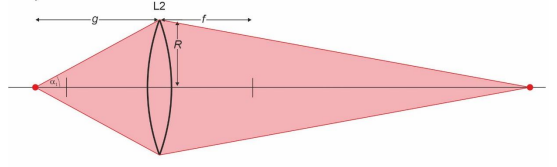
\includegraphics[width=0.5\linewidth]{nudes/NA-Skizze.png}
    \caption{Schematische Darstellung Bestimmmung NA \cite{teachcenter2}}
    \label{fig:NA-Skizze}
\end{figure}


\subsection{Variation der numerischen Apertur}

Der Einfluss des numerischen Apertur kann nur experimentell gezeigt werden, indem man sie variiert. Hierfür bietet es sich an, Linsen mit verschiedenen Durchmessern (Veränderung von R in \ref{eq:NA-umgeschrieben}) zu verwenden, oder der Einsatz einer Lochblende in der hinteren Brennebene der Linse.
Wie genau die numerische Apertur das Auflösungsverhalten beeinflusst wird im folgenden Experiment gezeigt.


\subsection{Abbesche Abbildungstheorie}

Wie im Kapitel Aufgabenstellung bereits einleitend erwähnt, besagt die Abbe Theorie, dass von jedem Objekt Beugungsmaxima hervorgehen und die Auflösung einen Zusammenhang zur Zahl der Beugungsmaxima besitzt.
Wichtig hierbei ist außerdem die Verwendung eines Gitters, dessen Spaltbreite dem halben Spaltabstand entspricht. Somit fehlen fehlen dem Gitter die gradzahligen Beugungsmaxima und am Bild hinter dem Vielfachspalt sind nur die ungradzahligen Maxima erkennbar (wird im Verlauf des Experimentes noch gezeigt).
Mit Hilfe des Tools für die grafische Darstellung solcher Muster von Leifi-Physik \cite{leifi} kann dieses Scenario theoretisch simuliert werden:

\begin{figure}[H]
    \centering
    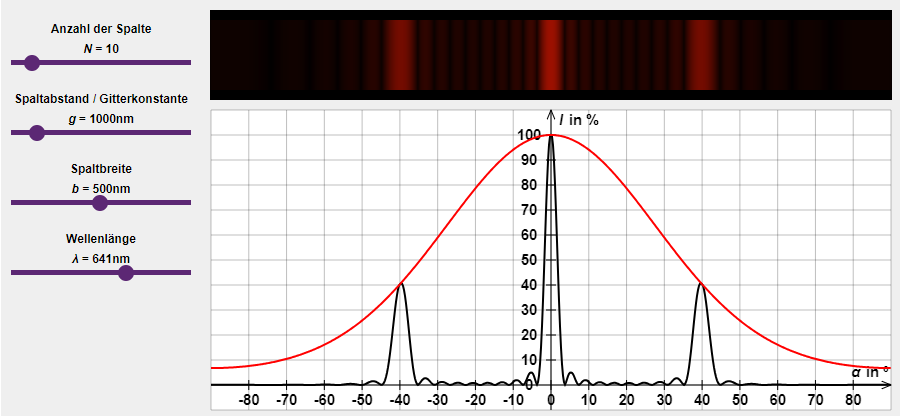
\includegraphics[width=0.4\linewidth]{nudes/VG-Simulation10Nrot.png}
    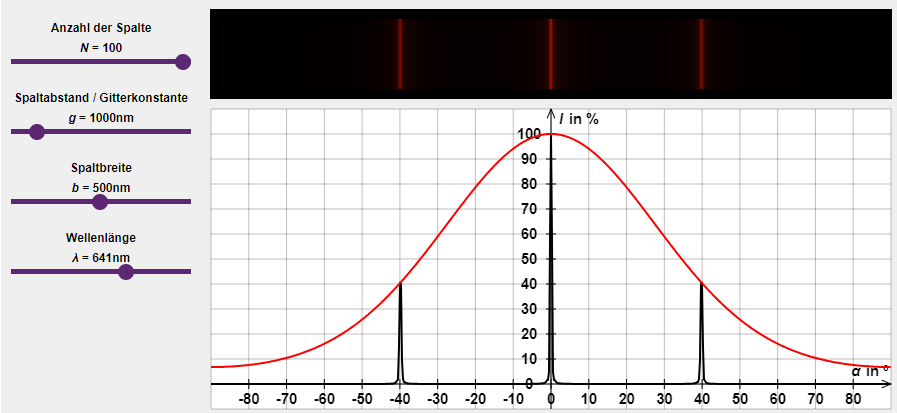
\includegraphics[width=0.4\linewidth]{nudes/VG-Simulation100Nrot.png}
    \caption{Simulation der Maxima einer Gitterbeugung von rotem Licht mit 10/100 Spaltöffnungen}
    \label{fig:SimulationRot}
\end{figure}

\begin{figure}[H]
    \centering
    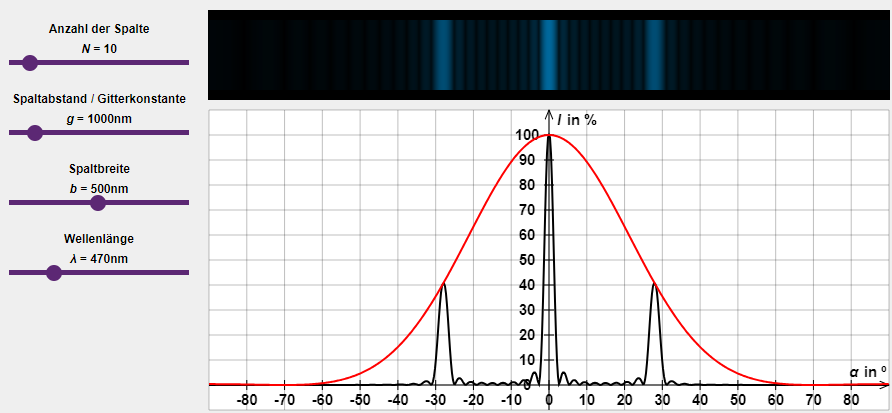
\includegraphics[width=0.4\linewidth]{nudes/VG-Simulation10Nblau.png}
    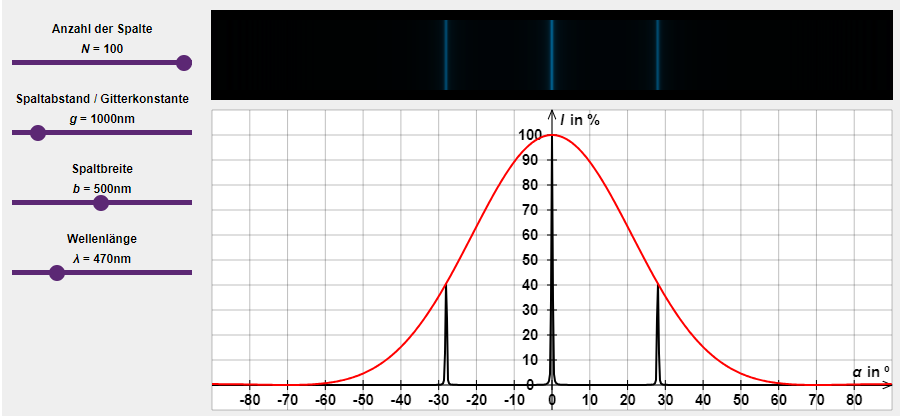
\includegraphics[width=0.4\linewidth]{nudes/VG-Simulation100Nblau.png}
    \caption{Simulation der Maxima einer Gitterbeugung von blauem Licht mit 10/100 Spaltöffnungen}
    \label{fig:SimulationBlau}
\end{figure}


\subsection{Wichtige Zusammenhänge}

Für eine erfolgreiche Auswertung der Daten werden außerdem folgende Zusammenhänge benötigt:

\begin{equation}
    \label{eq:WZ-NA}
    \centerline{Numerische Apertur \\ $NA = \frac{D_{Blende}}{2f_{2}}$ \\ $\Delta NA = \vert \frac{\partial NA}{\partial D_{Blende}} * \Delta D_{Blende} \vert + \vert \frac{\partial NA}{\partial f_{2}} * \Delta f_{2} \vert $}
\end{equation}

\begin{equation}
    \label{eq:WZ-dTheo}
    \centerline{Auflösungsvermögen theoretisch \\ $d_{theoretisch} = 0.61\frac{\lambda}{NA}$ \\ $\Delta d_{theoretisch} = \vert \frac{\partial d_{theoretisch}}{\partial \lambda} * \Delta \lambda \vert + \vert \frac{\partial d_{theoretisch}}{\partial NA} * \Delta NA \vert $}
\end{equation}

\begin{equation}
    \label{eq:WZ-fr}
    \centerline{Räumliche Frequenz \\ $f_{R} = 2^{n_{g}^{\frac{n_{E}-1}{6}}}$ \\ $\Delta f_{R} = \vert \frac{\partial f_{R}}{\partial n_{g}} * \Delta n_{g} \vert + \vert \frac{\partial f_{R}}{\partial n_{E}} * \Delta n_{E} \vert $}
\end{equation}

\begin{equation}
    \label{eq:WZ-dExp}
    \centerline{Auflösungsvermögen experimentell \\ $d_{experimentell} = \frac{1}{f_{R}}$ \\ $\Delta d_{experimentell} = \vert \frac{\partial d_{experimentell}}{\partial f_{R}} * \Delta f_{R} \vert$}
\end{equation}


    

\section{Versuchsanordnung} %mit skizze kurz beschreiben ------------------------------

Der Aufbau des Experimentes ist im Grunde sehr simpel. Es besteht aus einer Aluschiene, auf der acht verschiedene Module in einem bestimmten Abstand angebracht sind. 

\begin{figure}[H]
    \centering
    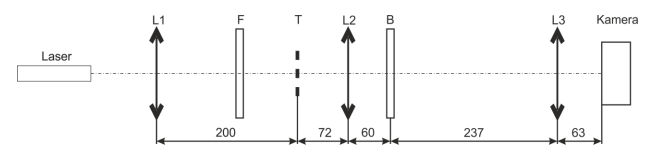
\includegraphics[width=0.8\linewidth]{nudes/VersuchsaufbauTheoretisch.png}
    \caption{Optischer Aufbau des Experiments; L1: f1 = 200mm, F: Filterrad mit roter/blauer LED, Graufilter und freiem
    Durchgang, T: Testobjekt; L2: f2 = 60mm; B: Filterrad mit 2/3/6 mm Lochblenden, einer Irisblende und einer
    Drahtblende, L3(einklappbar): f3 = 50mm. \cite{teachcenter2}}
    \label{fig:VersuchsaufbauTheoretisch}
\end{figure}

\begin{figure}[H]
    \centering
    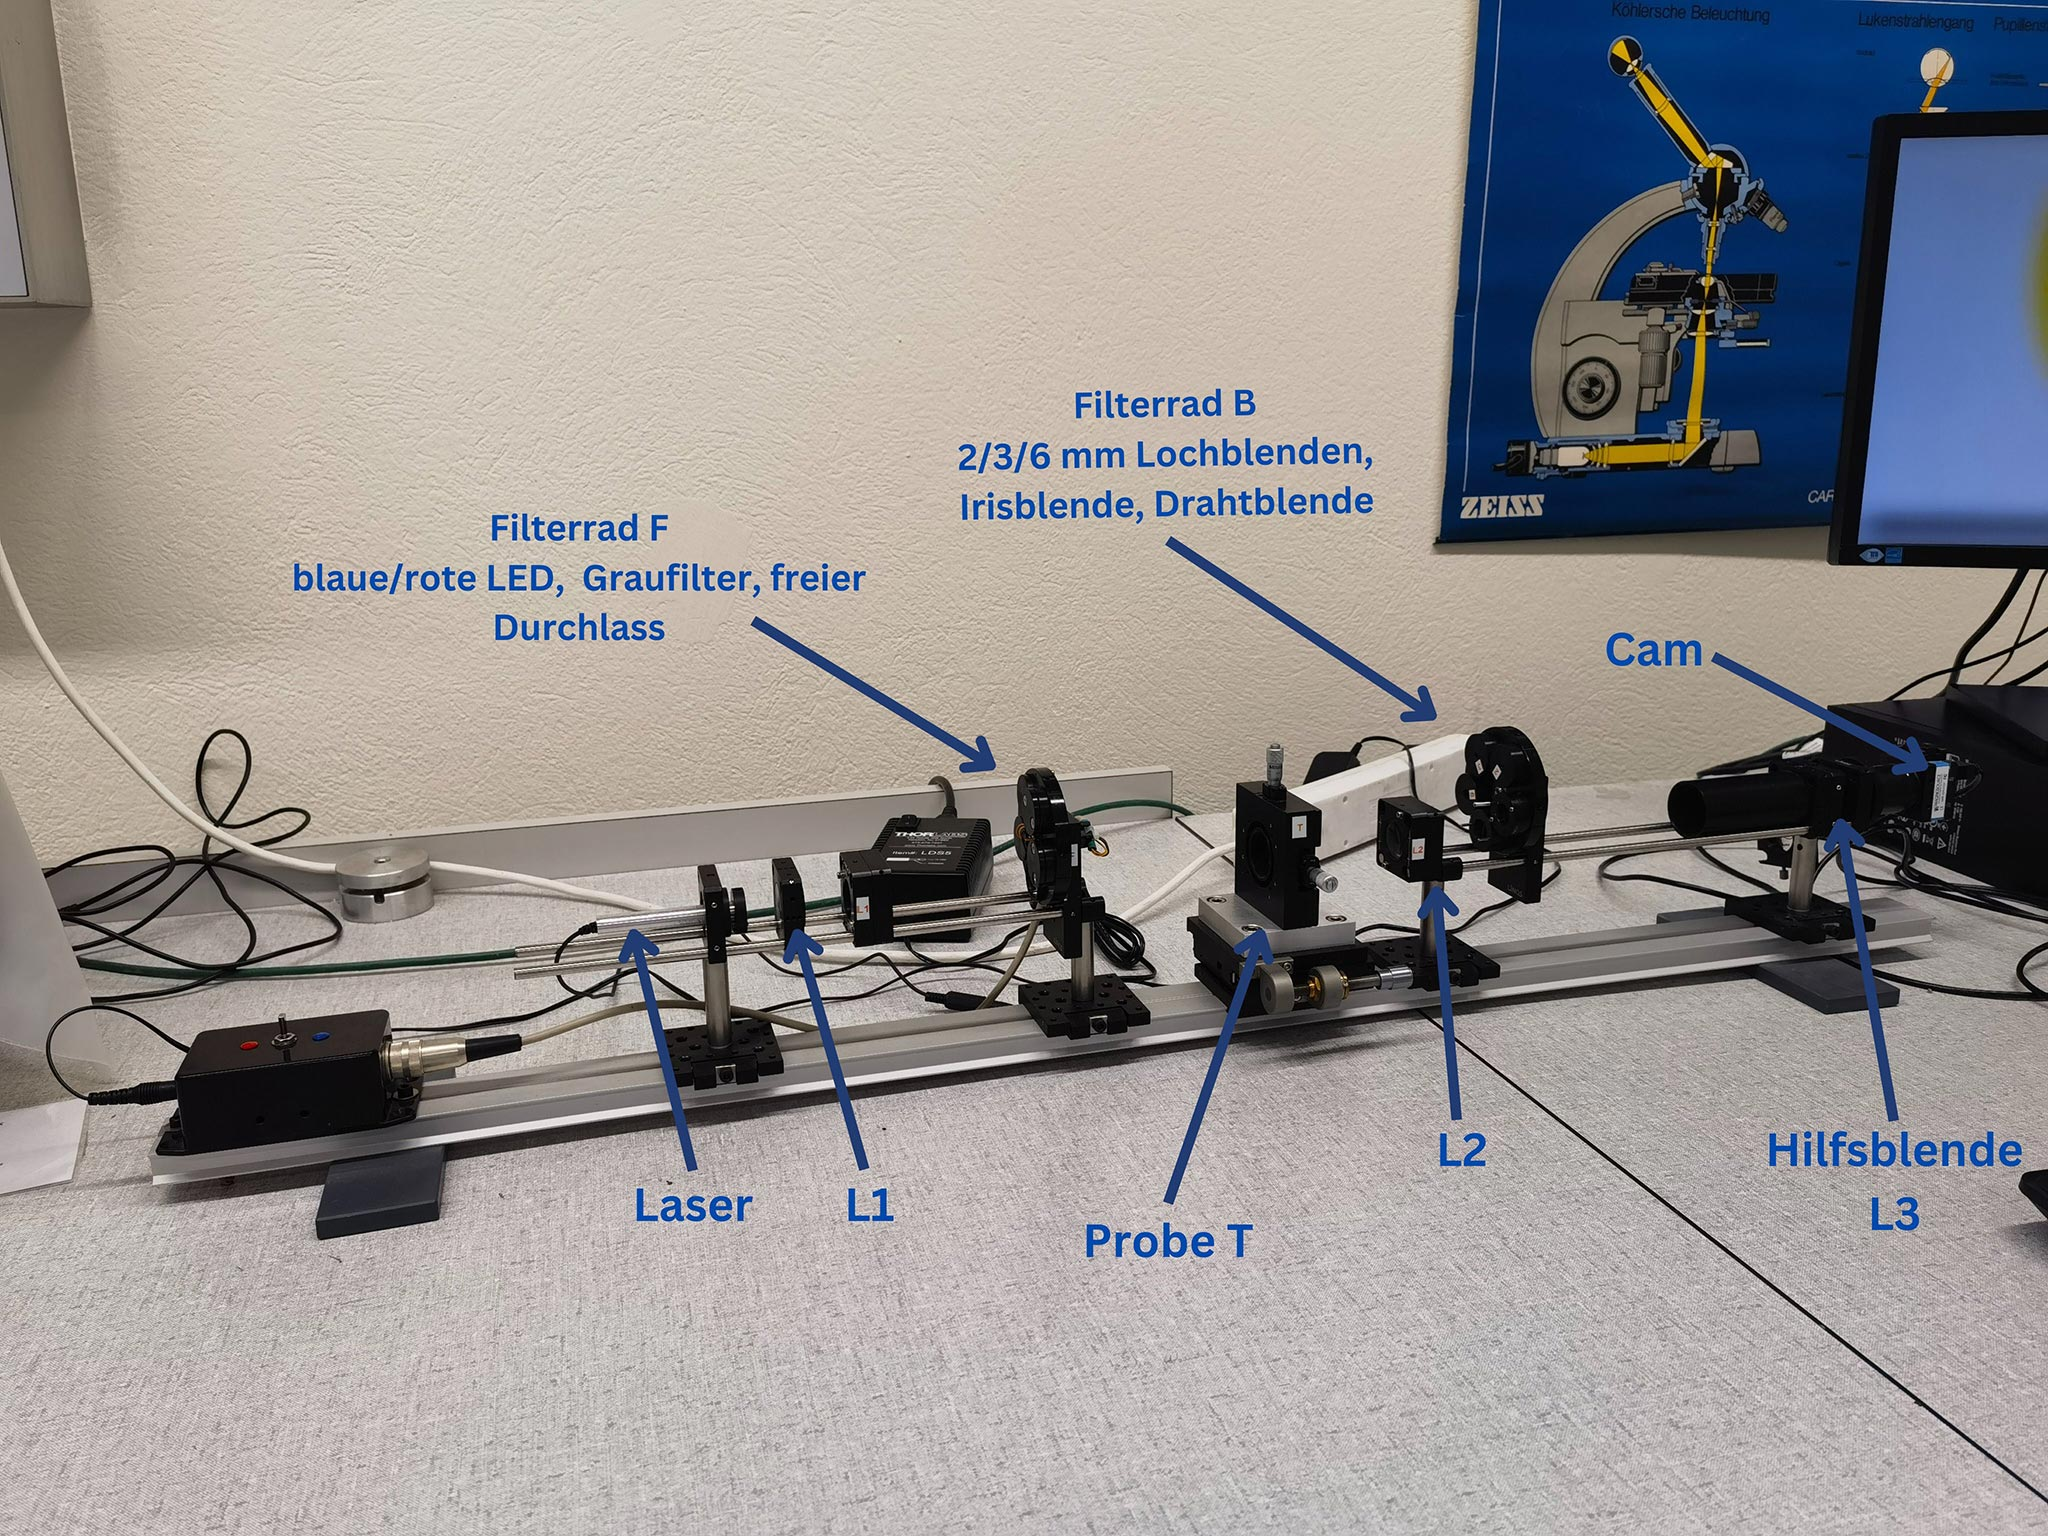
\includegraphics[width=0.7\linewidth]{nudes/VersuchsaufbauIRLbeschriftet.jpg}
    \caption{Versuchsaufbau laut Abbildung \ref{fig:VersuchsaufbauTheoretisch}}
    \label{fig:Versuchsaufbau}
\end{figure}

Die Einzelteile mit Beschreibung sind in folgender Tabelle ersichtlich:

\begin{table}[H]
    \centering
    \caption{Aufbau: Module}
    \label{tab:Aufbau}
    \begin{tabular}{| l | l | l | l |}
        \hline
        Nr.  & Modul & Bezeichnung  & Eigenschaft \\
        \hline
        1 & Laser & Laser & λ= 531,9 nm \\
        2 & Sammellinse 1 & L1 & f1 = 200 mm \\
        3 & Filterrad & F & rote/blauer LED, Graufilter und freier Durchgang \\
        4 & Testobjekt bzw. Probe & T &  \\
        5 & Sammellinse 2 & L2 & f1 = 60 mm \\
        6 & Filterrad & B & 2/3/6 mm Lochblenden, Irisblende und Drahtblende \\
        7 & Sammellinse 3 & L3 & f1 =  50 mm \\
        8 & Kamera & Kamera & Fotosensor mit PC/IC Capture Verbindung \\
        \hline
    \end{tabular}
\end{table}

\noindent
Teil der Vorbereitung war es auch, mögliche Strahlengänge durch diesen Aufbau theoretisch zu zeichnen. Diese sind in nachfolgenden Abbildungen zu sehen.

\begin{figure}[H]
    \centering
    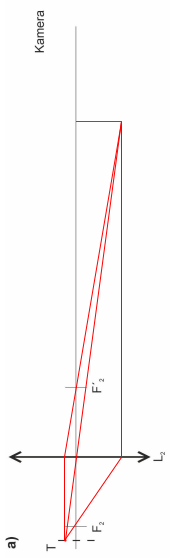
\includegraphics[width=0.3\linewidth, angle=-90]{nudes/Strahlenganga.png}
    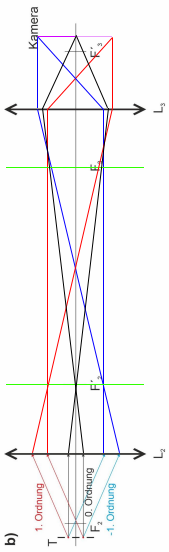
\includegraphics[width=0.3\linewidth, angle=-90]{nudes/Strahlengangb.png}
    \caption{Simulation der Maxima einer Gitterbeugung von blauem Licht mit 10/100 Spaltöffnungen}
    \label{fig:SimulationBlau}
\end{figure}

\section{Geräteliste} %jo holt a listn ------------------------------

    \begin{table}[H]
        \centering
        \caption{Im Versuch verwendete Geräte und Utensilien.}
        \label{tab:geraete}
        \begin{tabular}{| l | l | l | l | l |}
            \hline
            Gerät   & Bezeichnung  & Hersteller  & Eigenschaften  & Unsicherheit \\
            \hline
            Sammellinse & L1 & {n.a} & f1 = 200 mm & 1 mm \\
            Sammellinse & L2 & {n.a} & f1 = 60 mm  & 1 mm \\
            Sammellinse & L3 & {n.a} & f1 = 50 mm  & 1 mm \\
            Laser & Laser & Thorlabs & λ= 531,9 nm & {n.a.} \\
            LED blau & LEDb & Cxxx & λ= 470 nm & 5 nm \\
            LED rot & LEDr & Cxxx & λ= 635 nm & 5 nm \\
            Kamera & Kamera & The Imaging Source & {n.a.} & {n.a.}\\
            Kamera & {n.a.} & The Imaging Source & {n.a.} & {n.a.}\\
            SciDAVis & {n.a.} & Cxxx & {n.a.} & {n.a.} \\
            \hline
        \end{tabular}
    \end{table}


\section{Versuchsdurchführung \& Messergebnisse} %nachvollziehbar und klar dargestellt ------------------------------


\section{Auswertung und Unsicherheitsanalyse} %Nicht nur zahlen angeben ------------------------------

In der Auswertung werden zur erhöhten Genauigkeit durchgehend ungerundete Werte bis zu den Endergebnissen verwendet und nur zur Darstellung gerundet. \\
Zur Berechnung der Unsicherheiten wird, wenn nicht anders angegeben, die Größtunsicherheitsmethode verwendet.


\section{Diskussion} %diskussion der Unsicherheiten und Ergebnisse und evtl. verlgeich mit Literatur ------------------------------


\section{Zusammenfassung} %klare, übersichtliche vollständige beantwortung der Aufgabenstellung ------------------------------


\printbibliography[heading=bibintoc]
\end{document}
